	\section{Problem Formulation}
	\label{sec:gen}

	%% In this section we first discuss the nature of resolver's data.
	%% Then we propose a generative model that captures the essence of our understanding of per-user request generation.
	%% Finally we describe the process which interleaves the queries generated by different users and form the final resolver queue. 
	
	%% \subsection{Nature of Data}
	%% \label{subsec:nature}
	%% Here we provide an example that summarize the details of the nature of real data based on which we present our generative model in the following sections.	


	A user starts by visiting a page e.g., {\tt a.com}. While
        launching the webpage, many queries are being generated from
        different components of that browsed webpage: {\tt a.com, ad1.com,
        audio1.org}.  We refer to this sequence as a {\em query episode}.
% which happens during \emph{webpage} loading.
%        Other than the page's domain name a.com, other requested
%        domains may be related to the content of the webpage or
%        personalized for the user. 
        Next, when the user opens a new website another episode 
        is started.  The same process generates query
        sequences for other users.  For example, a second user generates: 
        {\tt b.com, ad2.com} and after the interleaving we may observe the
        following sequence in the resolver:{\tt  b.com, a.com, ad1.com,
        ad2.com, audio1.org}.
%	After issued by the user, each query is going to be enqueued into the local resolver's queue.
%	Because of different arrival time of a user's request, they get mixed with the other users' queries. 
	We call this process \emph{request interleaving}.
	Our goal is to deinterleave the two request sequences. 
	
	%	\section{Generative Model}	
	\subsection{User's Request Generation Model}
	\label{subsec:user}
	The \emph{browsing process} of a user can be modeled as simple
        as a Markov chain (MC) of webpages, an HMM, or an HsMM model.
        Figure \ref{fig:hsmm} illustrates these three different user
        model.
	
	In this section we present a most detailed model that explains
        user requests generation based on the process elaborated in
        Section \ref{subsec:nature}.  We model the browsing process
        using a Hidden Semi-Markov Model (HsMM).  MC and HMM are
        special cases of this process.  The hidden layer of the HsMM
        consists of random variables $W$ representing the browsed
        webpages.  Note that pages are hidden because what we see are
        only the DNS requests.

% e.g., if we just look at the queue of the
%        example of Section \ref{subsec:nature} maybe the main pages
%        are b.com which has the link to a.com and ad1.com, both
%        queried after it.  Therefore, we don't know what page was
%        initially loaded and generated its following queries in the
%        queue.
	
	The page transition matrix is different for each user and is
        represented by the matrix $\P_u$.  
%The duration random
%        variable $D$ of the hidden layer is the number of queries 
%        requested by the page.  And finally, 
        The observed state of the HsMM is the domain name request $R$
        which will be put in the resolver queue.
	Note that the time between subsequent browsed pages (which is equal to the time spend in a page before moving to the next one) in reality is different from the duration parameter in our model.
	In real world data, each user spends an interval on a page but in our model since we are only interested in the order of queries, we only count the number of requests that the page will query from the resolver and represent it by the random variable $D$.
	So the duration parameter $D$ represents the number of outstanding requests from the current page.
	
	%	In real world data, the burst of query generation per page visit, generates queries that have nearby time. 
	%	In contrast, duration parameter of the HsMM, . 	
	
	Fig \ref{fig:hsmm2} shows the details of the model and Table \ref{tab:params} summarizes the model parameters.
	$\O_u(w, r)$  is the probability of submitting (outputting/observing) request $r$ on the webpage $w$, for the user $u$.	
	Conditional probabilities of the model are as follows:	
	\begin{figure}
	\centering
	\subcaptionbox{
		Markov Chain
	}{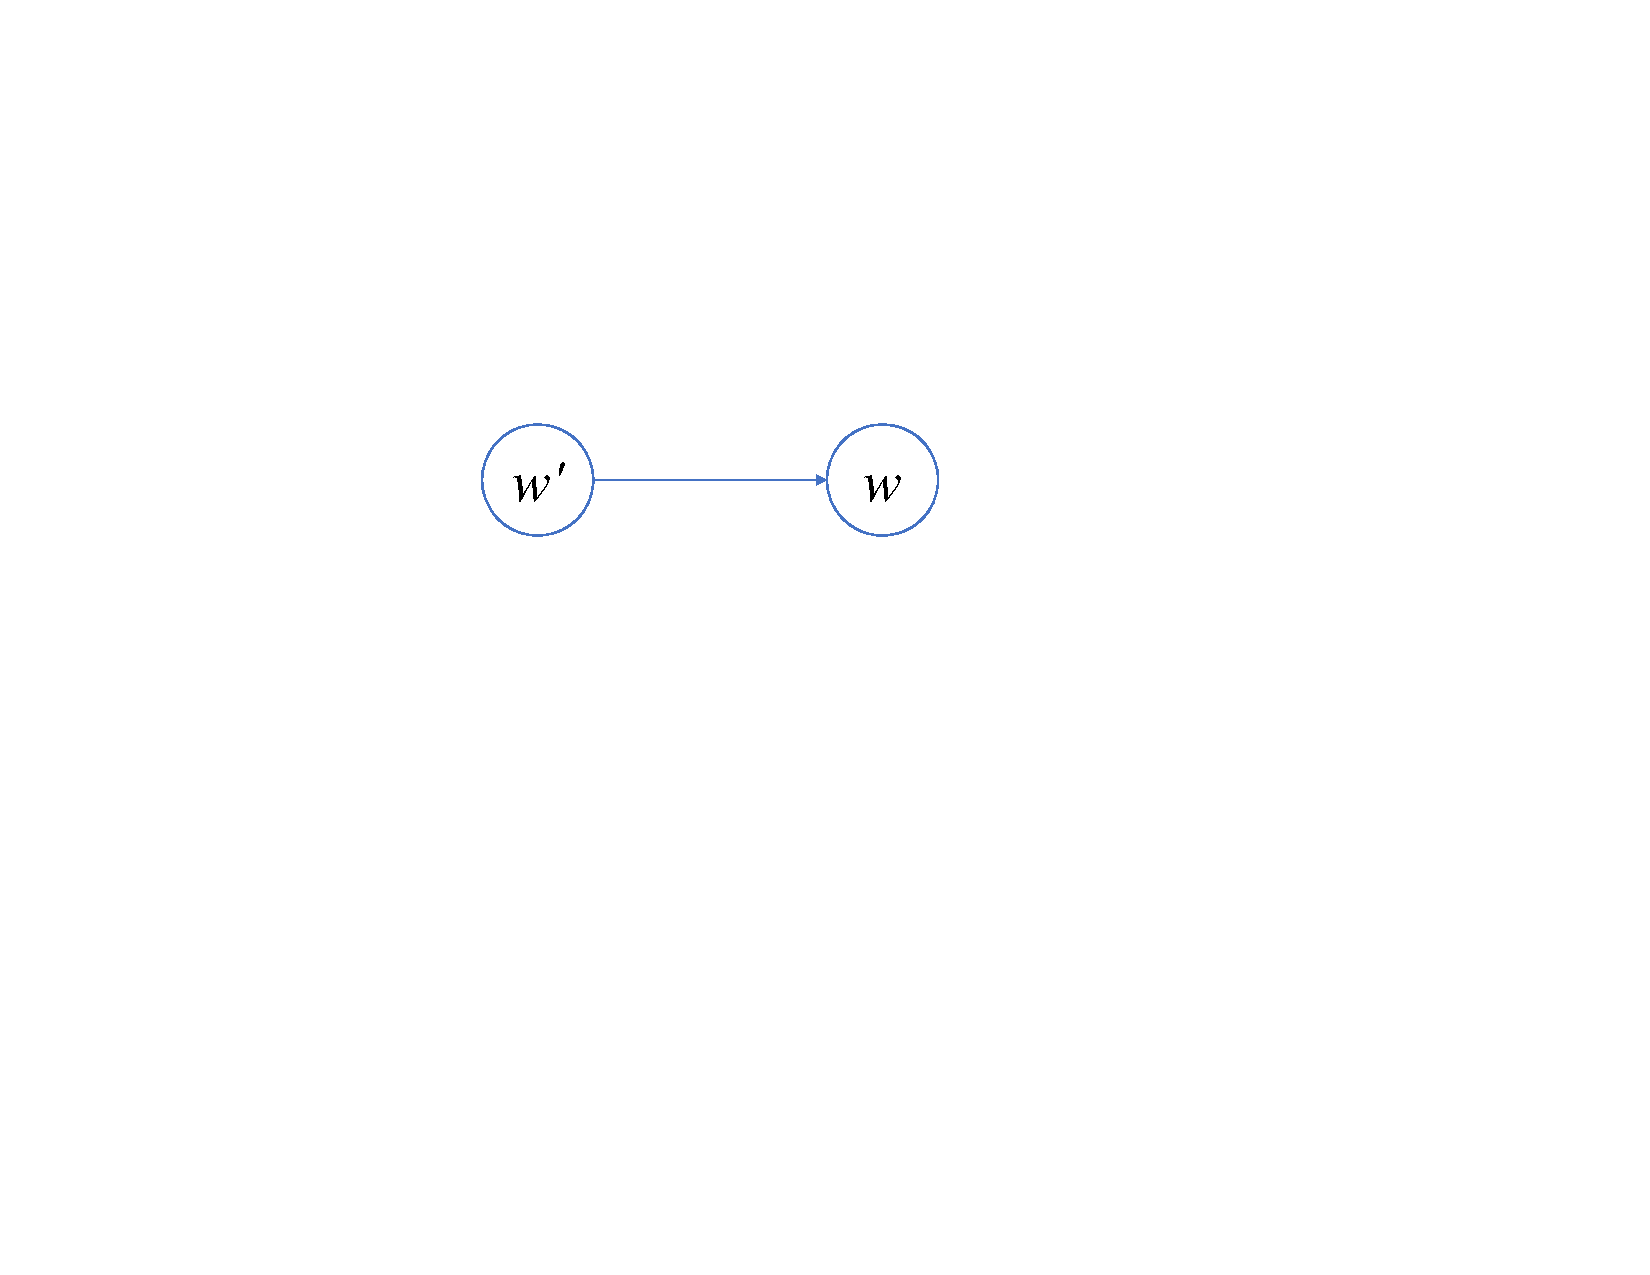
\includegraphics[width=0.14 \textwidth,]{./img/mc}}~
	\subcaptionbox{
		HMM
	}{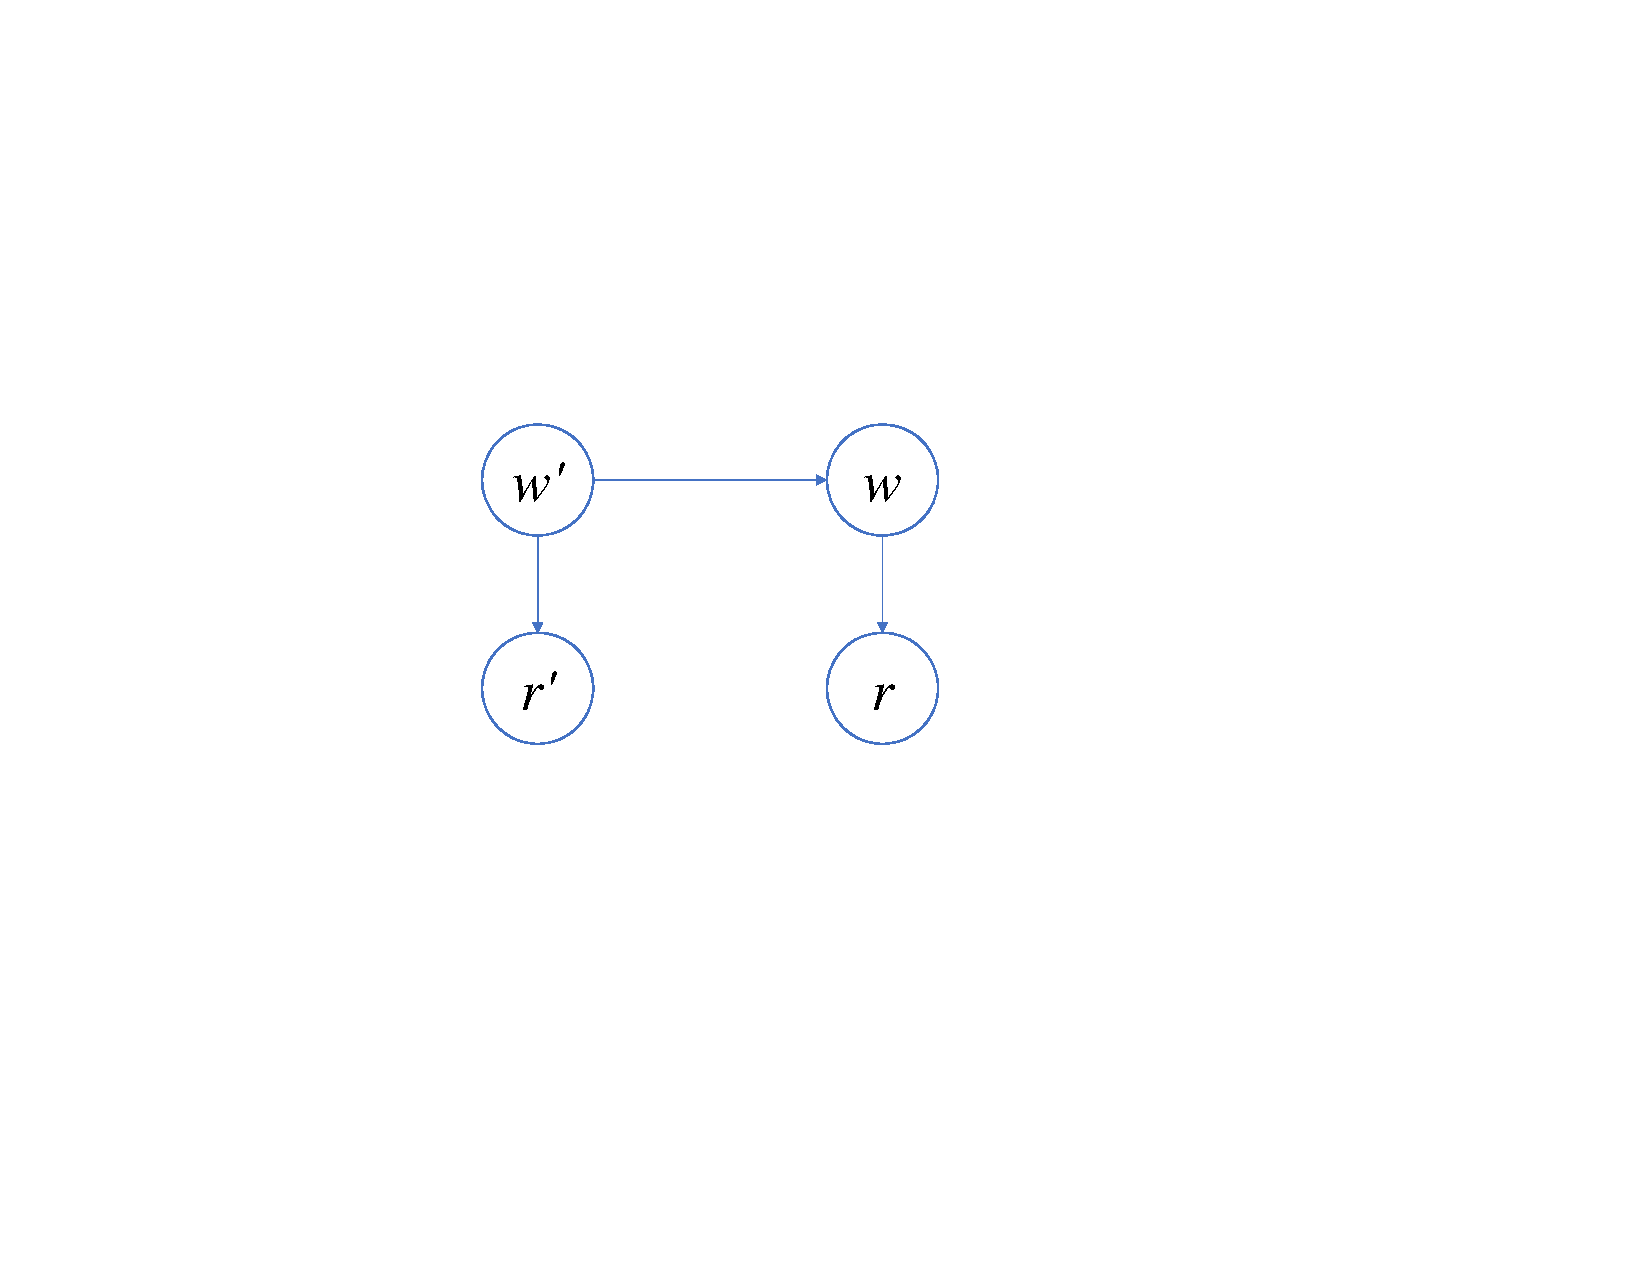
\includegraphics[width=0.14 \textwidth,]{./img/hmm}}~
	\subcaptionbox{
		HsMM
		\label{fig:hsmm2}
	}{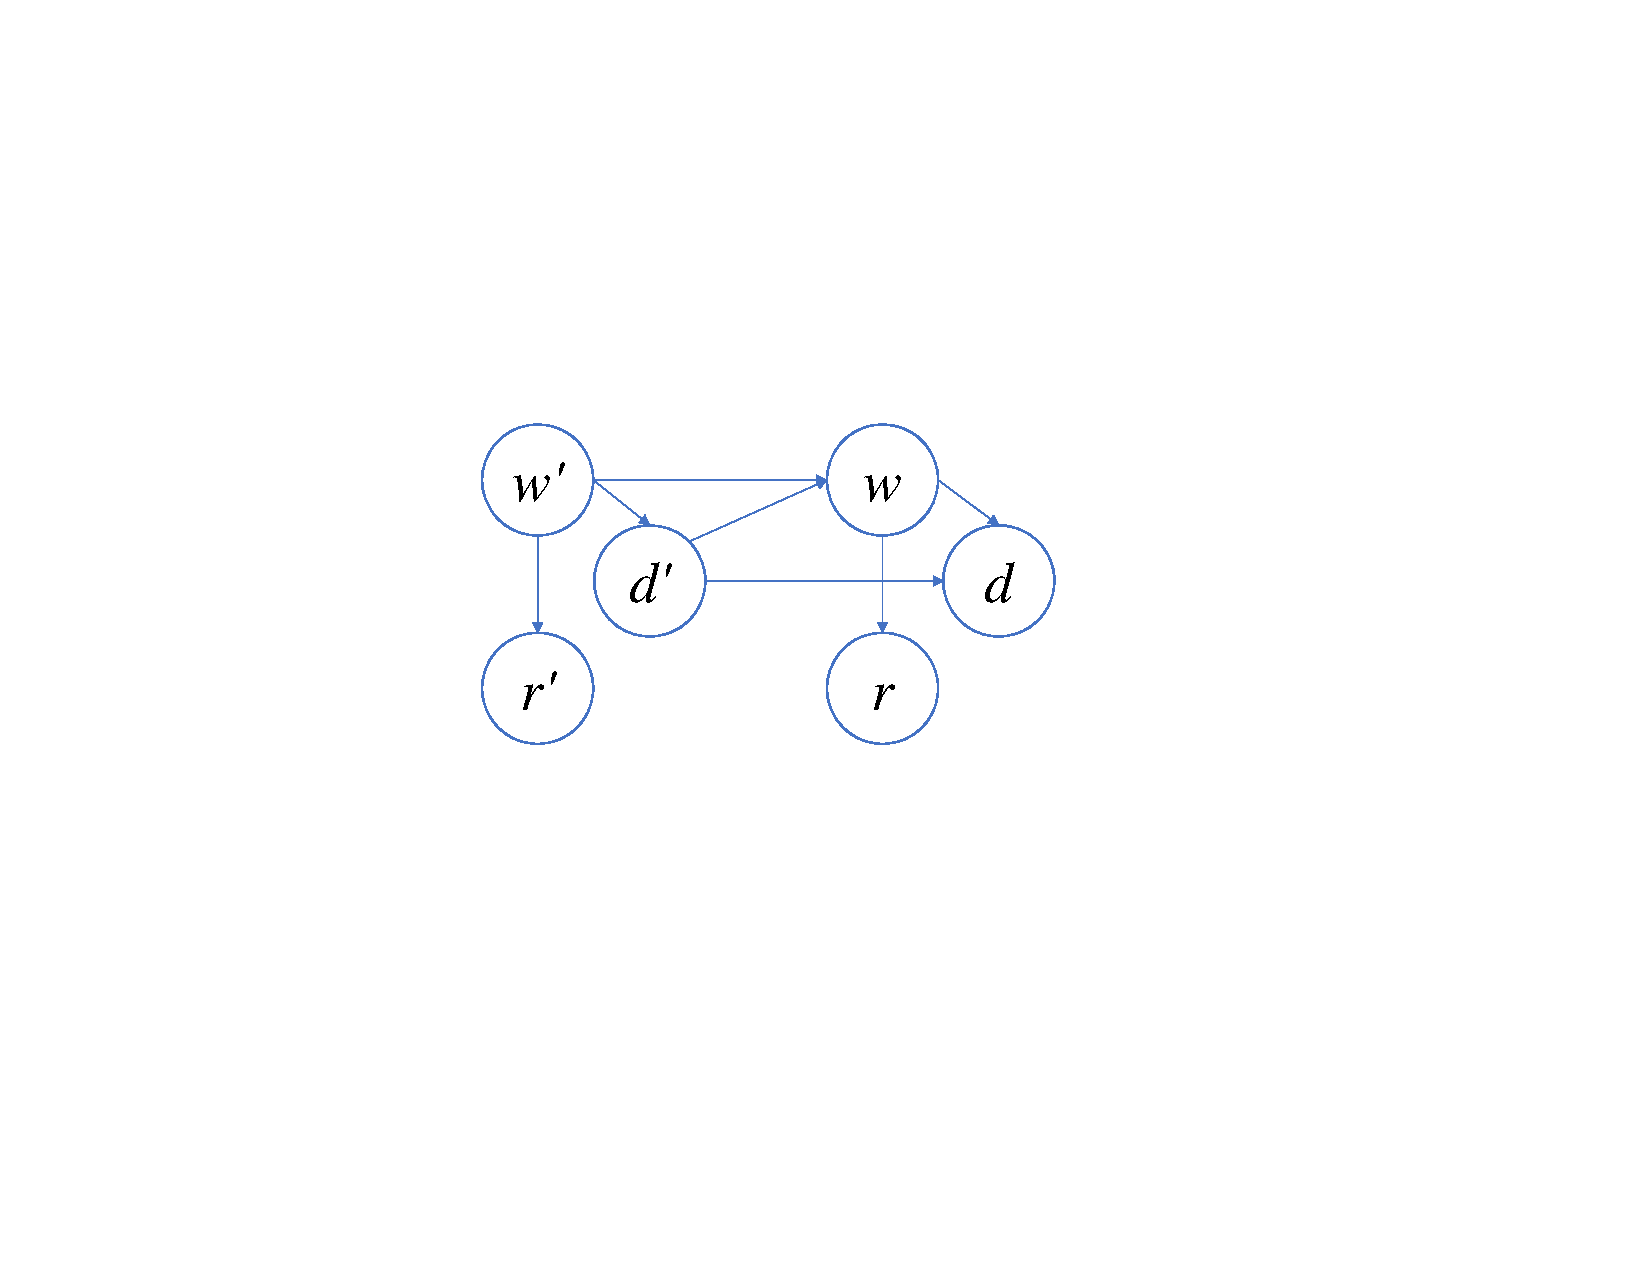
\includegraphics[width=0.17 \textwidth]{./img/hsmm2}}
	\caption{User's browsing models.}
	\label{fig:hsmm}
\end{figure}	
	
	
	
	\begin{equation}
	\label{eq:probs}
	\begin{alignedat}{3}
	\pr_u(w | w', d') &= 
	\begin{cases} 
	[\bP_u]_{w'w} & d' = 1  \\
	\delta(w, w') & d' > 1
	\end{cases} &,&
	\\ 
	\pr_u(d | w, d') &= 
	\begin{cases} 
	p_{w}(d) & d' = 1 \\
	\delta(d, d'-1) & d' > 1
	\end{cases} &,&
	\\   
	\pr_u(r|w) &= [\O_{u}]_{w, r}&,&	
	\end{alignedat} 
	\end{equation}
	
	The duration parameter cannot be zero, when $d = 1$ (i.e., the page's last request is submitted) and the user moves to another page which resets the duration using $p_w(d)$. 
	The duration probability $p_w(d)$ determines the number of requests that the webpage $w$ will query and is independent of user $u$. 
	%	Also, the output probability $\o_{w}(r)$ only depends on the webpage $w$. 
	
	\begin{table}
		\centering
		\begin{tabular}{|c|l}
			\hline
			Symbol & Explanation \\ 
			\hline 
			%$U$ & Random variable for the active user \\ \hline
			$W$ & RV for the webpage \\ \hline
			$D$ & RV for the number of requests to be issued on a page \\ \hline
			$R$ & RV for the issued DNS request \\ \hline
			\hline 
			$m$ & Number of users \\ \hline
			$n$ & Total number of pages \\ \hline
			$q$ & Maximum number of requests per page \\ \hline 
			\hline 
			$\P_u \in \reals^{n \times n}$ & Webpage transition matrix of the user $u$ \\ \hline 
			$p_w(d), d \in [q]$ & Distribution of number of requests $d$ on the page $w$ \\ \hline 
			$\O_u \in \reals^{n \times n}$ & Output distribution matrix of the user $u$  \\ \hline
		\end{tabular}
		\caption{Summary of the model parameters and random variables (RV). For each random variable the corresponding small letter represents a realization. Note that $W$ and $D$ depend on the user but to avoid cluttering we omitted the index $u$.}
		\label{tab:params}
	\end{table}
	
	\subsection{Resolver's Sequence Interleaving Model}
	\label{subsec:interle}
	As mentioned in Section \ref{subsec:nature}, we have access only to the resolver data queue where users enqueued their domain name requests. 
	Here we assume that there is a Markov chain governing the ``turn'' of users. 
	Let's assume that we have $m$ users.
	We name the transition matrix of the user's Markov chain as $\A = [\alpha_{ij}] \in \reals^{m \times m}$.
	Therefore the probability of user $j$ generating the $t$-th request given the current user as $i$ is $\pr(U(t)=j|U(t-1)=i) = \alpha_{ij}$.
	The random variable $U(t) \in [m]$ represents the active user that has generated the $t$th request of the resolver queue. 
	
	%	We define the interleaving process as follows.
	%	To generate the $t$-th request, first we should determine the active user and then a user $i$ is selected to generate the $t$th request in the resolver queue with probability $\alpha_i$. 
	%	More formally, the random variable $U(t)$ represents the user that generates the query at $t$th place of the resolver's queue. 
	A simplification of the transition matrix that has been used in literature is $\forall i, j: \pr(U(t) = i|U(t-1) = j) = \alpha_i$, where the whole dynamics of the system can be represented by a single user's \emph{shares vector} $\aalpha$ instead of the \emph{user's transition matrix} $\A$.
	
	To distinguish each user's corresponding HsMM random variable in the interleaving process we use both user index and time index. For example, $W_{k}(t)$ is the user $k$'s current webpage. 
	Note that here the time is different from the real world time and HsMM duration that discussed in Section \ref{subsec:user}. 
	Time here is just an index into the resolver's sequence of queries.
	For example, $W_{k}(t)$ shows the webpage of user $k$ when the $t$th request was submitted to the resolver. 
%	Note that, the $t$th request may have been generated by any of the users not only $k$. 
	
	We model the interleaving process as an Augmented Hidden Markov Model (AHMM), where the hidden states are augmented states, i.e., combination of variables \cite{minot2014separation}. 
	To make the equations more readable, we lump together the variables corresponding to each user and make the following lumped variable $L_k(t) = (W_{k}(t), D_{k}(t))$ and the hidden state of the HMM becomes $H(t) = (L_1(t), \dots, L_m(t), U(t))$ which is a $2m +1$ dimensional vector.
	Fig \ref{fig:rq} illustrates the interleaving process that leads to sequence generation.
	For simplicity, we assume $u(t-1) = u'$ and $u(t) = u$ which means that users $u'$ and $u$ are active at time steps $t-1$ and $t$ respectively. 
	\begin{figure}
		\centering
		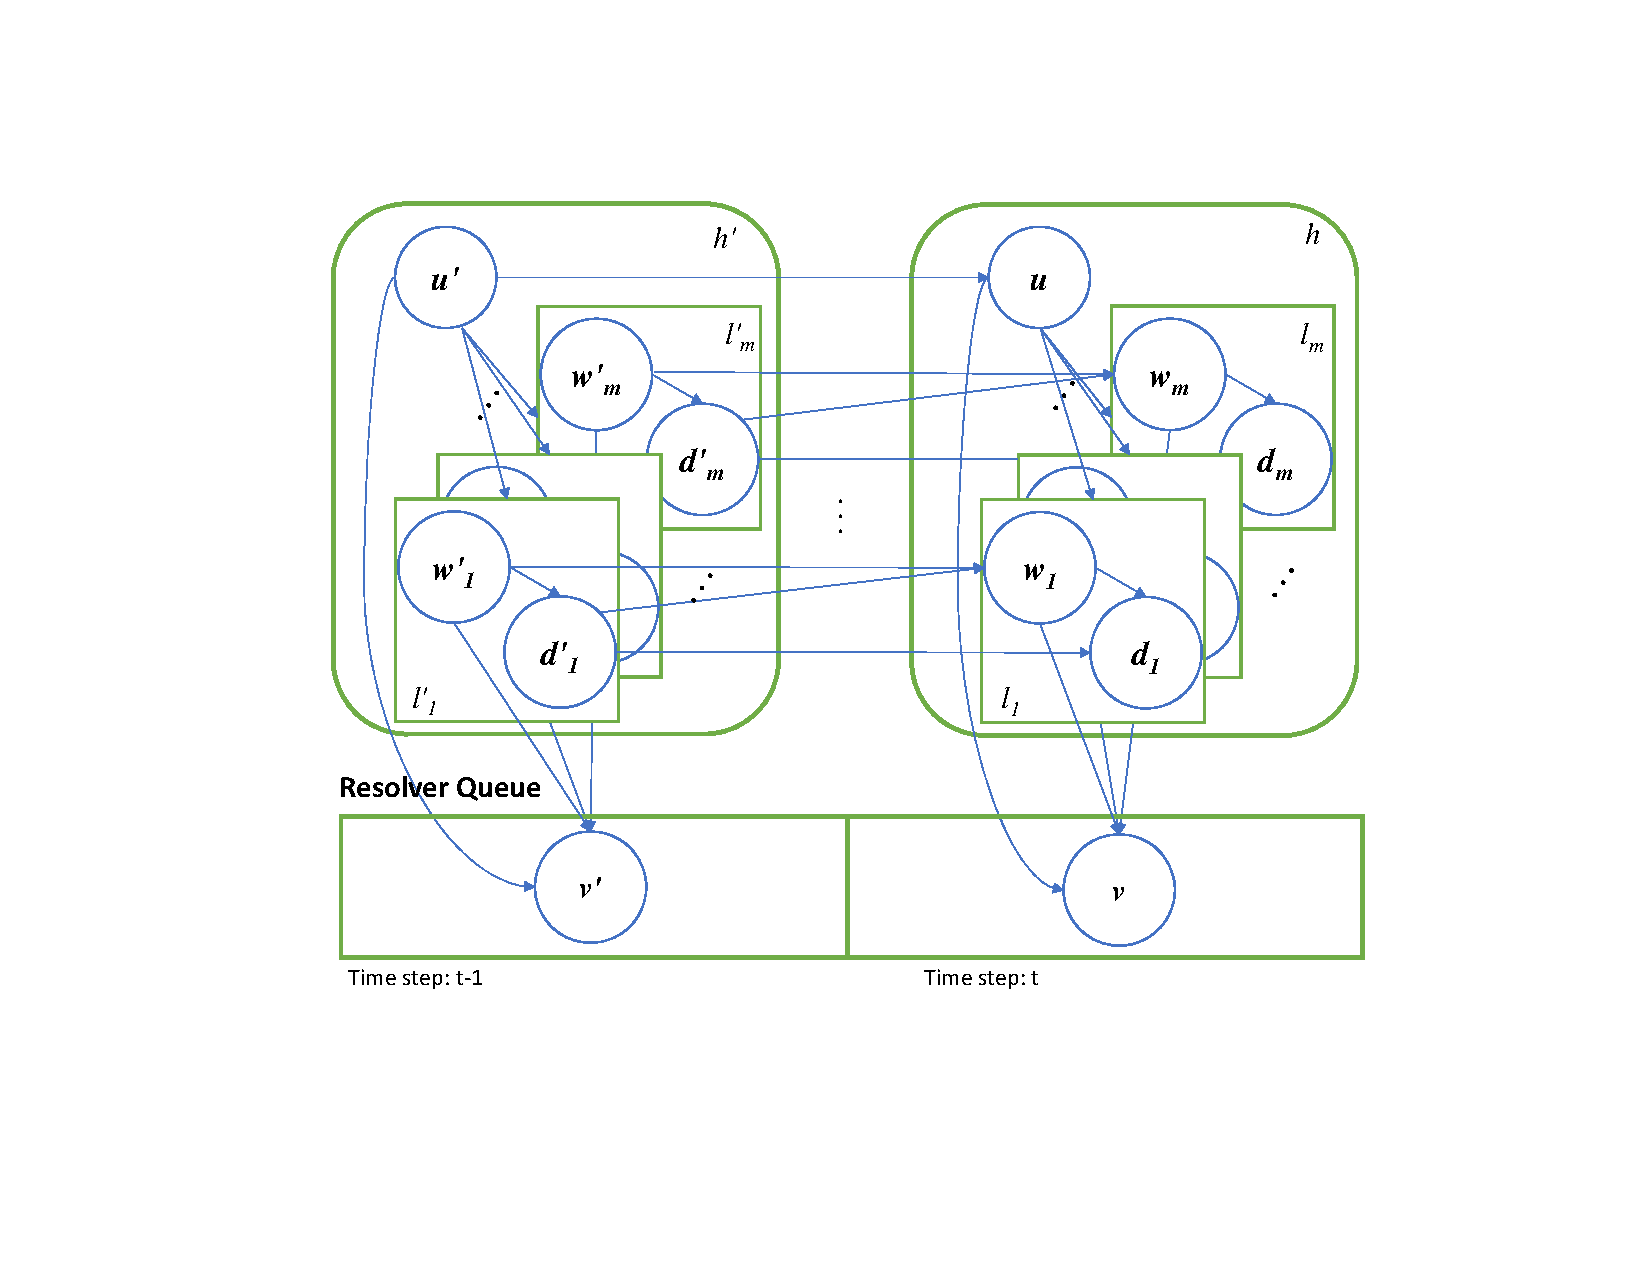
\includegraphics[width=.45\textwidth]{./img/hsmm-q2}
		\caption{Illustration of the interleaving process.}
		\label{fig:rq}
	\end{figure} 
	
	%Let's name the $t$th request in the queue as  at the time step $t$.  
	At the time step $t$, user $u(t) = u \in [m]$ generates the request $v(t)$ which is the observed (visible) variable of the HMM.
	The request $v(t)$ is determined by the next request of the user in its HsMM model, i.e., $r_{u}(t)$.	
	Therefore, the emission probability of the AHMM is:

	{\small
	\be 
	\nr 
	\pr(V(t) = v(t) | H(t) = h(t)) = \pr_{u}(r_{u}(t) | w_{u}(t)) = \O_{u}(w_{u}(t), r_{u}(t)).
	\ee 
	}
	%	Note that the emission probability is still only a function of the page $w$ but to keep track of each users current page we introduced $u$ as an index $w_u$, meaning that we are looking at the page that is browsed by user $u$. 
	%	We call the emission probability matrix that is built from $\o$s (in a way that is describe below) as $\E$.
	%	From now on, we omit the time index of $u(t)$ to avoid cluttering.
	Now we derive the entries of the transition probability matrix of the AHMM:
	\be 
	\pr(H(t) | H(t-1)) = \alpha_{u'u} \prod_{k=1}^{m} \pr(l_k(t) | l_k(t-1), u),
	\ee 
	%	where 
	%	\be
	%	\pr(l_k(t) | l_k(t-1), U(t) = u) = 
	%	\begin{cases}
	%		\pr_u(x | x', s') \pr_u(s | x, s') & u = k\\
	%		\delta(x, x')\delta(y, y')\delta(s, s')\delta(r, r') & u \neq k
	%	\end{cases}
	%	\ee 
	%	where $U(t) = j$. 
	In the case of $k \neq u$ the user $k$ is not active, i.e., stalled. 
	Substituting the probability distributions from \eqref{eq:probs}, we get: 
	\be
	\pr(l_k(t) | l_k(t-1), u) = 
	\begin{cases}
		k \neq u & \delta(w, w')\delta(d, d') \\
		k = u & 
		\begin{cases}
			d = 0 & p_w(d) [\P_u]_{w'w} \\
			d > 0 & \delta(d, d-1)
		\end{cases}  		
	\end{cases}
	\ee 
	
	\begin{table}
		\centering
		\begin{tabular}{|c|l|}
			\hline
			Symbol & Explanation \\ 
			\hline 
			$L$ & The lumped random variable $L = (W, D)$. \\ \hline
			$H$ & The hyper-hidden state of the HMM $H = (L_1, \dots, L_m, U)$.\\ \hline
			$V$ & The visible state of the HMM which is the requested DN. \\ \hline 
		\end{tabular}
		\caption{Summary of the augmented variables. For each random variable the corresponding small letter represents a realization.}
	\end{table}
	
